\section{Visualizzazione Transazioni}

Tornando alla pagina Home, rimangono due bottoni nel menù di sinistra: "Your Transactions" e "Inbound Transactions".
Cliccando su di essi si apriranno, rispettivamente, le pagine per visualizzare le transazioni in uscita dal proprio account e quelle in entrata.

\begin{figure}[H]
    \centering
    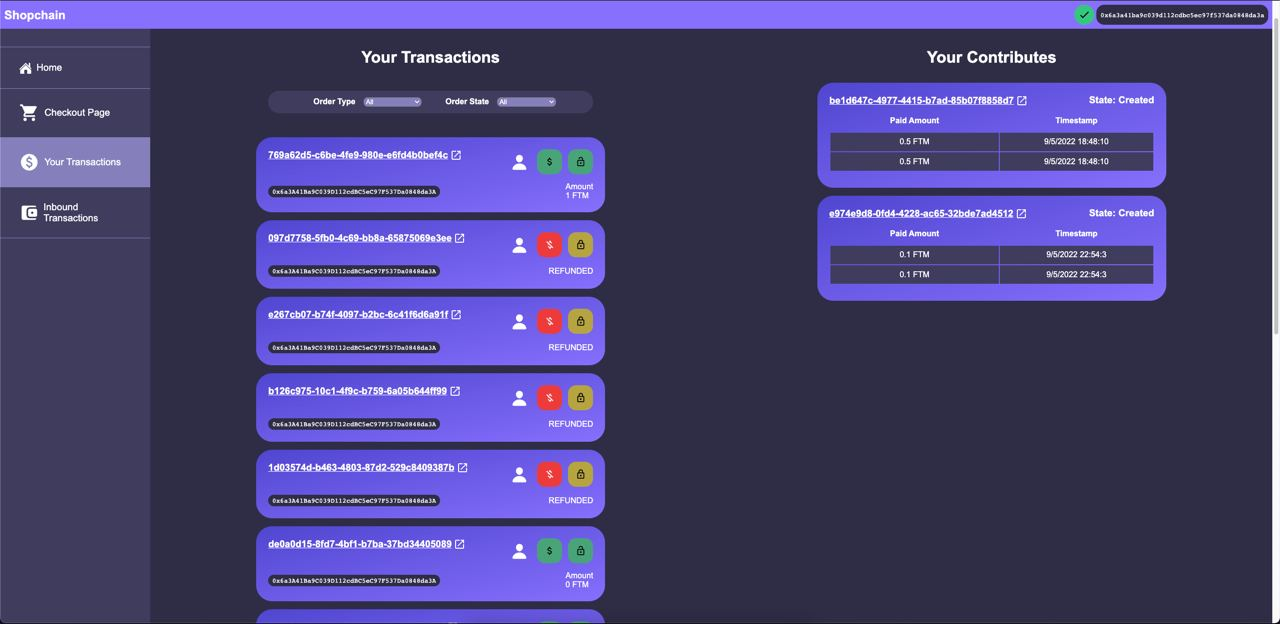
\includegraphics[scale=0.4]{immagini/transactionview.jpg}
    \caption{La vista delle transazioni in uscita}
\end{figure}

\subsection{Ordinamento transazioni}

L'applicazione offre la possibilità di ordinare l'elenco delle transazioni in due possibili modalità, combinabili tra loro: 
"Order Type", il tipo dell'ordine, e "Order State", lo stato corrente dell'ordine.
La scelta è effettuata tramite un apposito menu a tendina.

\begin{figure}[H]
    \centering
    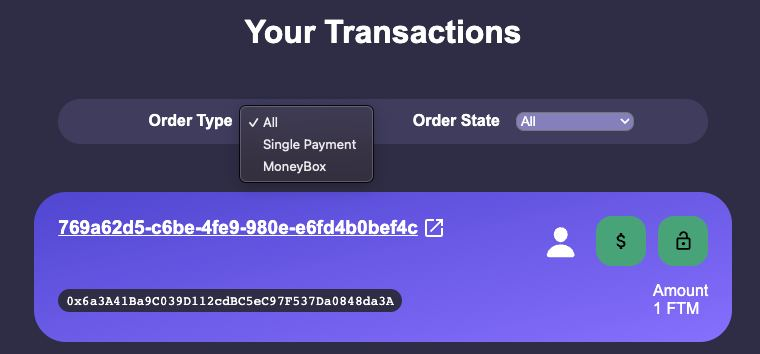
\includegraphics[scale=0.4]{immagini/ordertype.jpg}
    \caption{Menu per la scelta del tipo di ordine}
\end{figure}

Il tipo di ordine potrà essere:
\begin{itemize}
    \item All: tutti i tipi di ordine;
    \item Single Payment: pagamento singolo;
    \item MoneyBox: pagamento creato come MoneyBox dall'utente.
\end{itemize}

\begin{figure}[H]
    \centering
    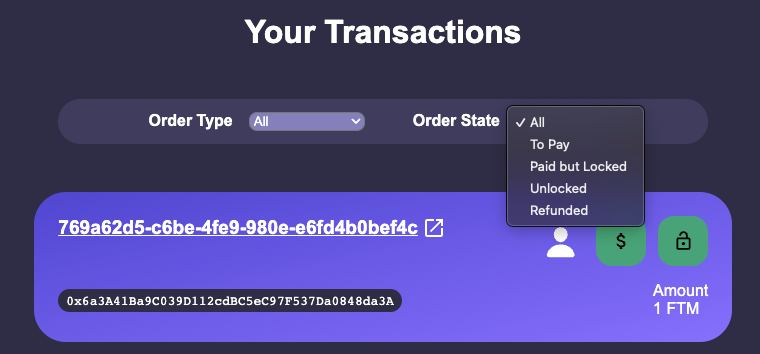
\includegraphics[scale=0.4]{immagini/orderstate.jpg}
    \caption{Menu per la scelta dello stato dell'ordine}
\end{figure}

Lo stato dell'ordine invece:
\begin{itemize}
    \item All: tutti i tipi di stato;
    \item To Pay: il pagamento deve ancora essere completato;
    \item Paid but Locked: il pagamento è stato effettuato interamente, ma non ancora sbloccato;
    \item Unlocked: il pagamento è stato effettuato e sbloccato;
    \item Refunded: il pagamento è stato rimborsato.
\end{itemize}

%come settare account seller